%/**
% * LaTeX thesis template (main file)
% * @author  : Alexander willner (willner@cs.uni-bonn.de)
% */

% /* include config ------------------------------------------------------ */
\newcommand{\metaFilename}{thesis_template}
\input{\metaFilename.config.tex}
%\excludecomment{finalComments}
\def\showDedication{1} % 1=show it, 0=hide it
% /* --------------------------------------------------------------------- */


% /* begin paper --------------------------------------------------------- */
\begin{document}
    %\frontmatter
    \pagestyle{empty}
    \pagenumbering{alph}
    \begin{titlepage}
\rmfamily
\begin{flushleft}
%%\begin{center}
\LARGE{\textbf{\metaTitle}}\\
\normalsize

\vspace{1,4cm}
%\textbf{\metaType}\\
%\metaWhy\\
%\metaArticle~hier stand metaFaculty
\metaFaculty\\
%\metaArticle~ hier stand metaUniversity
\metaUniversity\\

\vspace{1,4cm}
\metaSubmitted\\
\textbf{\metaAuthor}, %\textbf{\metaDegree}\\
%\metaBirthplace\\

\vspace{1,4cm}
\metaCity, \metaDate\\

\vspace{1,4cm}
%Some \\
%more \\
%Text.\\

\vspace{1,4cm}
\hspace{-.4cm}
\begin{tabular}{ll}
First reviewer & : \metaFirstReviewerName \\
Second reviewer & : \metaSecondReviewerName \\
Day of submission & : \metaDateExam
\end{tabular}
%%\end{center}
\end{flushleft}

%\setlength{\wpYoffset}{40pt}
%\ThisLROffsetCornerWallPaper{.2}{resources/images/logo}

\end{titlepage}

    %\cleardoublepage
    %%/**
% * LaTeX thesis template (deposition)
% * @author  : Alexander willner (willner@cs.uni-bonn.de)
% */

\vspace*{100mm}
\begin{minipage}{109.5mm}
\section*{Affidavit}
I hereby declare that the following thesis "\metaTitle" has been
written only by the undersigned and without any assistance from third
parties.\\

Furthermore, I confirm that no sources have been used in the preparation
of this thesis other than those indicated in the thesis itself.\\[2cm]
\metaCity, \metaDate
\end{minipage}

   % \ifnum\showDedication > 0
   % \cleardoublepage
      %%/**
% * LaTeX thesis template (dedication)
% * @author  : Alexander willner (willner@cs.uni-bonn.de)
% */

\pdfbookmark{Dedication}{dedication}
\begin{center}
\Large{\metaDedication}
\end{center}

    %\fi
    %\cleardoublepage

    \pagestyle{headings}
    \pagenumbering{roman}
    \setcounter{page}{1}
    %/**
% * LaTeX thesis template (abstract)
% * @author  : Alexander willner (willner@cs.uni-bonn.de)
% */
\pdfbookmark{Abstract}{abstrct}
\chapter*{Abstract}\label{sec:abstract}
%\mtcaddchapter\addcontentsline{toc}{chapter}{Abstract}


\sidenote{Introduction and Problem Statement}
%\textit{Introduction and Problem Statement:}
Continuous and broad innovation in the Information- and Communications sector has extensively changed the way that communication takes place between peers during the last years, as well as it has changed who and how services are provided to users. The rapid growth in data traffic demand and an increasing competitive pressure has decreased profits for telecommunication-network providers and has resulted in overall value chain challenges.
To go along with altered market requirements and conditions a new technological approach had to be found.

\textit{Related Work and Research Questions:}
Current telecom infrastructure consists of a large amount of heterogeneous network elements such as routers, gateways, firewalls, policy control and so on. Orchestrating these elements to work together to rapidly create a new service is demanding if not nearly impossible. Semi-automatic creation and management of application layer services must be orchestrated in accordance with constraints or policies of the underlying network infrastructure. 
SDN in conjunction with VNF is about to cope with this challenge. SDN and NFV can be seen as a new network architecture paradigm applying new technological capabilities to network functions, network design and service platforms in order to achieve agile, flexible, scalable and efficient networks, which will help to lower management costs and OPEX in the long run.  
The OASIS TOSCA standard defines a metamodel for defining IT services. It introduces the concept of a “service template” which defines both the structure of a service (“topology”) as well as how to manage it (“orchestration”). The generic service template describes what needs to be preserved when an application is migrated over alternative network or cloud environments. This ensures interoperability of deployment and management throughout the complete service lifecycle.
On the other side, members from IT and telecoms industries are currently working to develop standards for Network Functions Virtualisation (ETSI NFV). Early implementations demonstrate that network design itself has to be more agile instead of having an ever increasing variety of proprietary hardware with single, dedicated functions. Instead the network needs to be able to respond instantaneous to the dynamic needs of the traffic and services running over it. 
%\lipsum[6]

\textit{Own Approach:}
To establish a direct and reliable linkup between both the ETSI and OASIS data models can be a tedious task if one of the standards definitions change and a running system implementation needs to be adapted each time. Most likely some kind of changes will occur in future evolution. Hence there is a distinct need for an intermediary solution which will work independent of current data model specification. This can be done through a REST-paradigm approach and the usage of “Plain Old Java Objects” (POJOs) which will act as a robust bridge in-between both data model domains to ensure a hitch-free information flow.

\textit{Research Contributions:}
The main contributions of this thesis will be a concept (approximately 40 pages) and the development of a RESTful application Interface prototype which will implement the functionality to convert  TOSCA information into POJOs and vice versa. All functions will be implemented with the aid of Java API for RESTful Web Services (JAX-RS).

\newpage


\begin{figure}
	\centering
		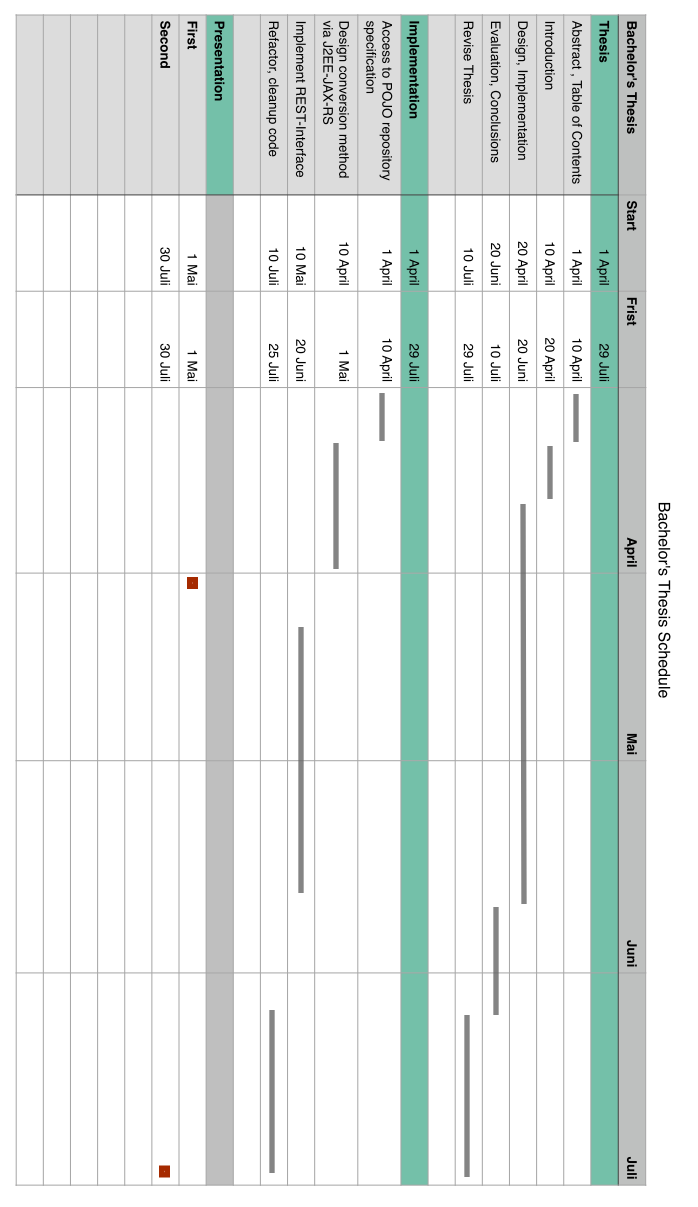
\includegraphics[width=0.93\textwidth]{resources/images/schedule.png}
	\label{fig:schedule}
\end{figure}



%\sidenote{Outlook}


%    \begin{quote}
%    "`\begin{CJK}{UTF8}{gbsn}不闻不若闻之,闻之不若见之,见之不若知之,知之不若行之;学至于行之而止矣。\end{CJK}"' -
%    \textit{Xunzi, Chinese philosopher (about 300-230 BC)}
%
%    "`not hearing is not as good as hearing, hearing is not as good as
%       seeing, seeing is not as good as mentally knowing, mentally knowing is
%       not as good as acting; true learning continues up to the point that
%       action comes forth [or, only when a thing produces action can it be said
%      to have been truly learned]"'
%    \end{quote}

%\cleardoublepage
%\chapter*{Zusammenfassung}\label{sec:zusammenfassung}
%\sidenote{Einleitung und Problemstellung}
%\lipsum[6]

%\sidenote{Verwandte Arbeiten und Forschungsfragen}
%\lipsum[6]

%\sidenote{Wissenschaftlicher Beitrag}
%\lipsum[6]

%\sidenote{Zusammenfassung}
%\lipsum[6]
\cleardoublepage

    \ifnum\showDedication > 0
    %%/**
% * LaTeX thesis template (ackknowledgment)
% * @author  : Alexander willner (willner@cs.uni-bonn.de)
% */

\pdfbookmark{Acknowledgments}{ack}
\chapter*{Acknowledgments}
This template was conducted during my time as ...

First and foremost, I would like to thank ...

I would like to express special thanks to ...

\vspace{0.5in}
\begin{flushright}
  \metaCity, \metaDate
\end{flushright}

    \fi
    \cleardoublepage

    %\phantomsection
    %%/**
% * LaTeX thesis template (tables)
% * @author  : Alexander willner (willner@cs.uni-bonn.de)
% */

\pdfbookmark{Table of Contents}{toc}
\tableofcontents
%\mtcaddchapter\addcontentsline{toc}{chapter}{Table of Contents}
\cleardoublepage

\listoffigures
\mtcaddchapter\addcontentsline{toc}{chapter}{\listfigurename}
\cleardoublepage

\listoftables
\mtcaddchapter\addcontentsline{toc}{chapter}{\listtablename}
\cleardoublepage

\lstlistoflistings
\mtcaddchapter\addcontentsline{toc}{chapter}{List of Algorithms}
\cleardoublepage

\chapter*{List of Abbreviations and Symbols}
\mtcaddchapter\addcontentsline{toc}{chapter}{List of Abbreviations and Symbols}

\begin{acronym}[LLOONNGG]
\acro{SONA}{SO Neat Acronym}
\acro{SLA}{So Light Acronym}

\vspace{10 mm}
\acro{H2O}[$\mathrm{H_2O}$]{Water}
\end{acronym}
\cleardoublepage

    %\cleardoublepage

    %\mainmatter
   % \pagenumbering{arabic}
    %\setcounter{page}{1}
    %\linenumbers
    %%/**
% * LaTeX thesis template (introduction)
% * @author  : Alexander willner (willner@cs.uni-bonn.de)
% */

\cleardoublepage\chapter{Introduction}\minitoc\label{sec:introduction}\vspace{.5cm}
\sidenote{general introduction to the context and the core of the thesis}
\noindent\lipsum[7]

\section{Problem Statement and Research Questions}
\lipsum[7]

\section{Reasearch Contributions}
\lipsum[7]
\begin{itemize}
  \item[\textbf{Goal 1}:]
  \lipsum[5]

  \item[\textbf{Goal 2}:]
  \lipsum[5]

  \item[\textbf{Goal 3}:]
  \lipsum[5]

  \item[\textbf{Goal 4}:]
  \lipsum[5]
\end{itemize}

\section{Outline of the Thesis}
We conclude with an outline of the thesis and a short summary of each chapter.
\begin{itemize}
  \item[\textbf{\chaptername~\ref{sec:relatedwork}}:]
  \sidenote{related work}
  \lipsum[5]

  \item[\textbf{\chaptername~\ref{sec:assumptions}}:]
  \sidenote{assumptions}
  \lipsum[5]

  \item[\textbf{\chaptername~\ref{sec:concept}}:]
  \sidenote{concept}
  \lipsum[5]

  \item[\textbf{\chaptername~\ref{sec:evaluation}}:]
  \sidenote{evaluation}
  \lipsum[5]

  \item[\textbf{\chaptername~\ref{sec:summary}}:]
  \sidenote{summary}
  \lipsum[5]
\end{itemize}


    %%/**
% * LaTeX thesis template (related work)
% * @author  : Alexander willner (willner@cs.uni-bonn.de)
% */

\cleardoublepage\chapter{Related Work and Research Gaps}\minitoc\label{sec:relatedwork}\vspace{.5cm}
\sidenote{review of relevant work on different sub problems.}
\noindent\lipsum[7]

\section{Summary}
\lipsum[5]

    %%/**
% * LaTeX thesis template (assumptions)
% * @author  : Alexander willner (willner@cs.uni-bonn.de)
% */

\cleardoublepage\chapter{Assumptions, Objectives and Scope}\minitoc\label{sec:assumptions}\vspace{.5cm}
\sidenote{text}
\noindent\lipsum[7]

\section{Use Cases and Assumptions}
\lipsum[5]

\section{Requirements and Objectives}
\lipsum[5]

\section{Test}

\cite{Waitzman:1999}

\small
\begin{equation}
  \begin{array}{l}
    \displaystyle t^{p_d}_{fw}(d) = max_{d}(t_{child_{i}}) \\
    \displaystyle t^{p_d}_{db}(d) = \sum_{i=1}^{d} t_{db_{i}} \\
    \displaystyle t^{p_d}_{pc}(n,d) =
    	\begin{cases}
        	t_{pc}(d) + c(n) & \text{if $d = 1$,}\\
        	t_{pc}(d) + c(n) + max(t_{avail}(d)) & \text{if $d>1$.}\\
        \end{cases}
  \end{array}
  \label{eq:var_idb}
\end{equation}
\normalsize

\begin{figure}
    \centering
    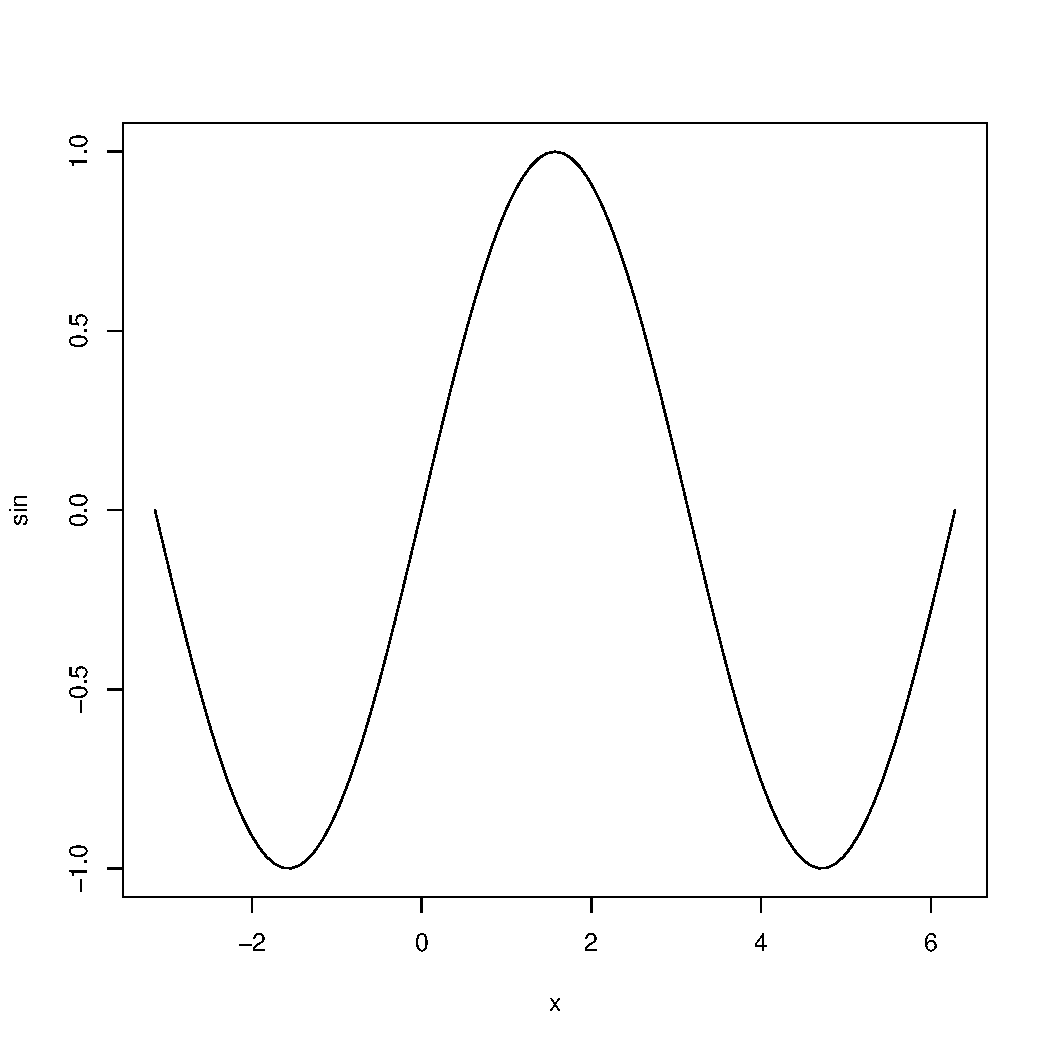
\includegraphics[width=.65\textwidth]{resources/images/example1.pdf}
    \caption{Example image.}
    \label{fig:example1}
\end{figure}

\begin{figure}
    \centering
    \subfloat[example2]{
        \label{fig:example2}
        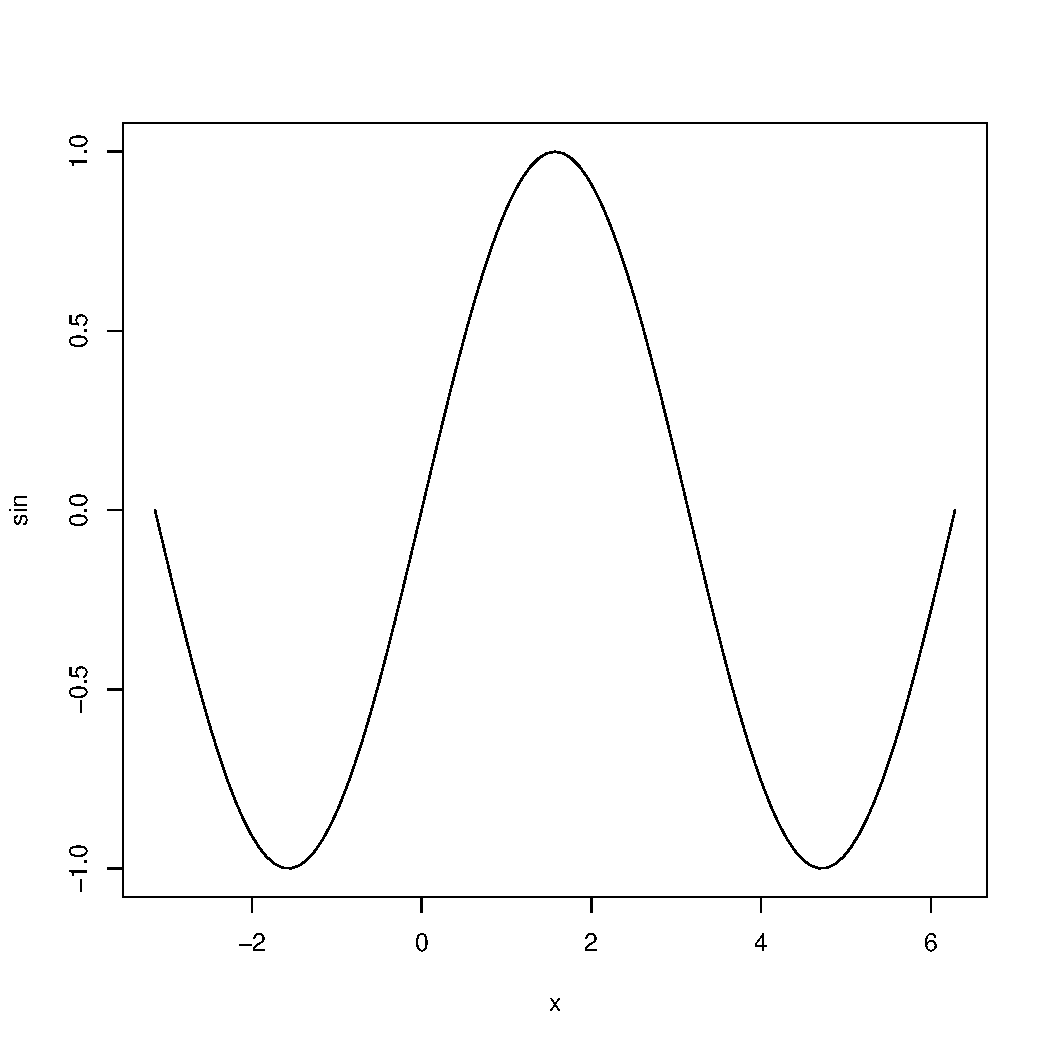
\includegraphics[width=.4\textwidth]{resources/images/example2.pdf}
    }
    \subfloat[example3]{
        \label{fig:example3}
        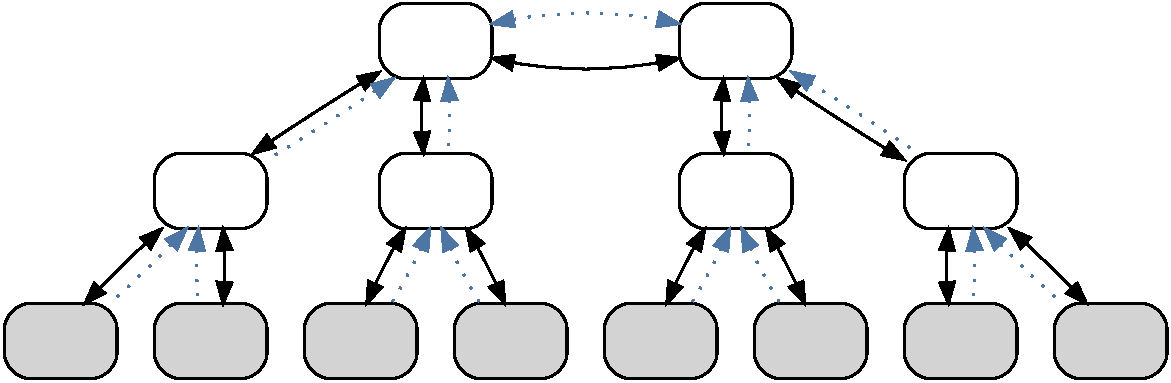
\includegraphics[width=.4\textwidth]{resources/images/example3.pdf}
    }
    \caption{Example images.}
    \label{fig:exammple2_3}
\end{figure}


\begin{center}
    \begin{longtable}{ll}
        \label{tbl:exampletable}\\
        \captionabove{Example table}\\
        \toprule\textbf{Name} & \textbf{Age}\\\midrule
        \endfirsthead
        \toprule\textbf{Name} & \textbf{Age}\\\midrule
        \endhead
        \midrule
            \multicolumn{2}{r}{\emph{Continued on next page}}
        \endfoot
        \bottomrule
        \endlastfoot
       Hans           & 80             \\
       Heinrich       & 77             \\
       Herbert        & 84             \\
    \end{longtable}
\end{center}

\lstset{language=Java, caption=Example Code., %
label=lst:example, numbers=left, stepnumber=1}
\lstinputlisting{resources/code/example.java}

\section{Summary}
\lipsum[5]

    %%/**
% * LaTeX thesis template (anaysis)
% * @author  : Alexander willner (willner@cs.uni-bonn.de)
% */

\cleardoublepage\chapter{Reseach Question 1}\minitoc\label{sec:concept}\vspace{.5cm}
\sidenote{Introduction and Problem Statement. Up to 40 pages.}
\noindent\lipsum[7]
\section{Related Work}
\sidenote{some text}
\label{sec:concept:relatedwork}
\lipsum[7]
\section{Own Approach / Concept / Contribution}
\sidenote{some text}
\label{sec:concept:approach}
\lipsum[7]
\section{Evaluation}
\sidenote{some text}
\label{sec:concept:evaluation}
\lipsum[7]

\section{Discussion}
\sidenote{some text}
\label{sec:concept:discussion}
\lipsum[7]
\section{Chapter Summary}
\sidenote{some text}
\label{sec:concept:summary}
\lipsum[7]

    %%/**
% * LaTeX thesis template (evaluation)
% * @author  : Alexander willner (willner@cs.uni-bonn.de)
% */

\cleardoublepage\chapter{Performance Evaluation}\minitoc\label{sec:evaluation}\vspace{.5cm}
\sidenote{simulation environment, metrics, parameter}
\noindent\lipsum[7]

\section{General Model}\label{sec:model}
\lipsum[5]

\section{Considered Metrics}\label{sec:metrics}
\lipsum[5]

\section{Analytical Evaluation}\label{sec:analytic}
\lipsum[5]

\section{Simluative Evaluation}\label{sec:sim}
\lipsum[5]

\section{Chapter Summary}\label{sec:result}
\sidenote{Lessons learned and transferability}
\lipsum[5]


    %%/**
% * LaTeX thesis template (summary)
% * @author  : Alexander willner (willner@cs.uni-bonn.de)
% */

\cleardoublepage\chapter{Conclusions, Discussions and Future Work}\minitoc\label{sec:summary}\vspace{.5cm}
\sidenote{Reference to problem, listing from inferences, sorted from important to unimportant. About 2--4 pages. We're now on page 140.}
\noindent\lipsum[7]

\section{Results}
\sidenote{Listing of the scientific contributions and what is new}
\label{sec:summary:results}
\lipsum[7]

\section{Deployability}
\sidenote{On how the results can be used}
\label{sec:summary:deployability}
\lipsum[7]

\section{Future Work}
\sidenote{Open research questions}
\label{sec:summary:futurework}
\lipsum[7]


    %\nolinenumbers
    %\cleardoublepage

    %\appendix
    %\pagenumbering{Roman}
    %\setcounter{page}{1}
    %%/**
% * LaTeX thesis template (appendix)
% * @author  : Alexander willner (willner@cs.uni-bonn.de)
% */


\cleardoublepage\chapter{Formal Description of Something}\minitoc\label{sec:formal}\vspace{.5cm}
\sidenote{Some appendix.}
\noindent\lipsum[7]

\cleardoublepage\chapter{Some more Evaluation Results}\minitoc\label{sec:moreeval}\vspace{.5cm}
\sidenote{Some appendix.}
\noindent\lipsum[7]

    %%/**
% * LaTeX thesis template (unsorted)
% * @author  : Alexander willner (willner@cs.uni-bonn.de)
% */

\cleardoublepage\chapter{\LaTeX~Tests}\minitoc\label{sec:latextest}\vspace{.5cm}
\sidenote{Some unsorted \LaTeX~tests}
\noindent\lipsum[7]

\begin{itemize}
  \item[\textbf{Acronyms}:] \ac{SONA} again \ac{SONA}. And \acp{SLA} also \ac{SLA} again \acp{SLA}. And \acf{SLA}.
  \item[\textbf{Index}:] Index\index{Index} and Subindex\index{Index!Subindex} in the \appendixname.
  \item[\textbf{Mote annotations}:] \ac{H2O}.
\end{itemize}




    %\cleardoublepage
    %\bibliographystyle{abbrv}
    %% To list uncited references (disable the line above):
    %\bibliographystyle{unsrt}
    %\cite{uncited}
    %\nocite{*}

    %\bibliography{\metaFilename,build}
    %\mtcaddchapter\addcontentsline{toc}{chapter}{Bibliography}

    %\backmatter
    %\cleardoublepage
    %\renewcommand{\indexname}{Index}
   % \printindex
\end{document}
% /* ----------------------------------------------------------- end paper */
